\chapter{Field Content of the Standard Model}
\label{chap:Field}

The \ac{SM} of particle physics is a quantum field theory that combines the concept of classic field theory with quantum mechanics and Einstein's special relativity. Different fundamental particles can be described as the excited states or quanta of distinct quantum fields, characterized by masses and various quantum numbers. A summary of the known fundamental particles and their properties is given in Figure~\ref{fig:Field}.

\begin{figure}[tbh!]
 \begin{center}
 \begin{tabular}{c}
 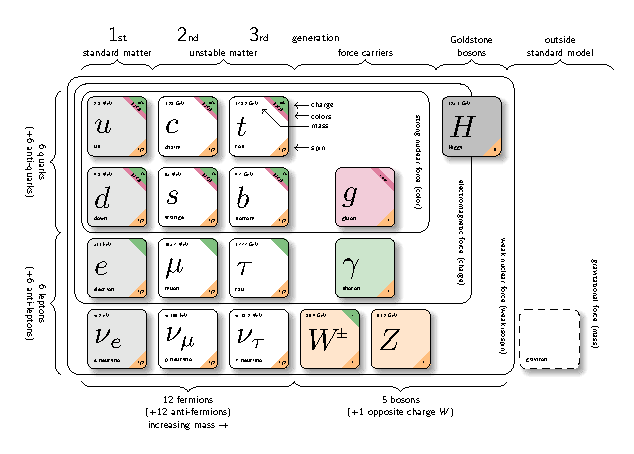
\includegraphics[width=\textwidth]{figures/Part1/Field/SM}
 \end{tabular}
 \caption{The field content of the \ac{SM}, including all known fundamental particles. The three generations of fermions are shown in the first three columns. The gauge bosons that mediate the fundamental interactions are shown in the fourth and fifth columns. The sixth column shows the recently discovered Higgs boson. The hypothetical graviton that mediates gravitational force is also shown, which is outside of the realm of the \ac{SM}.~\cite{tikz:SM}}
 \label{fig:Field}
 \end{center}
\end{figure}

The effects described by special relativity apply to all fundamental particles. This requires the theory to be invariant under Lorentz transformations, which contain rotations and Lorentz boosts of the coordinate systems. The behaviors of fundamental particles under such transformations are characterized by their spin quantum numbers. This divides fundamental particles into two groups. Those with half-integer spins are known as ``fermions''. They are fundamental building blocks of matter that exist in the universe. Particles with integer spins are known as ``bosons''. They are either mediators of the fundamental forces or are required in the mechanism that generates mass for all fundamental particles. Properties of elementary fermions and bosons are discussed further in \autoref{sec:Fermion} and \autoref{sec:Boson}, respectively. 

\section{Fermions}
\label{sec:Fermion}

Named after Italian physicist Enrico Fermi, fermions follow Fermi-Dirac statistics and obey the Pauli exclusion principle, which prohibits two or more fermions with the same quantum number from simultaneously occupying the same quantum state. The matter that exists in the universe is made up of spin-$\frac{1}{2}$ fermions that can be broken into two groups, quarks and leptons. They are represented by ``spinors'' under Lorentz transformations. For example, the free Lagrangian that encodes full information of a spinor field can be expressed as,

\begin{equation}
\label{eq:lefthand}
\mathcal{L}=i\psi_{R}^{\dagger}\sigma^{\mu}\partial_{\mu}\psi_{R}
\end{equation}
or
\begin{equation}
\label{eq:righthand}
\mathcal{L}=i\psi_{L}^{\dagger}\bar{\sigma}^{\mu}\partial_{\mu}\psi_{L},
\end{equation}

where $\sigma^{\mu}$ is the 2$\times$2 Pauli matrix. The spinors in Equation~(\ref{eq:lefthand})-(\ref{eq:righthand}) are known as Weyl spinors, which correspond to two-dimensional irreducible representations of the Lorentz group. Weyl spinors can be classified into left-handed spinors $\psi_{L}$ or right-handed spinors $\psi_{R}$ depending on the orientation of their spin relative to their momentum. More formally, $\psi_{R}$ and $\psi_{L}$ correspond to the ($\frac{1}{2}$,0) and (0,$\frac{1}{2}$) representation of the Lorentz group~\cite{zee:group}.

In addition to Lorentz invariance, the free Lagrangians should also be invariant under parity transformation. For Weyl spinors, however, this symmetry is violated as right-handed spinors transform into left-hand spinors under parity, and vice versa. To describe elementary fermions, the two irreducible representations must be stacked together, forming a four-dimensional reducible representation ($\frac{1}{2}$,0) $\bigoplus$ (0,$\frac{1}{2}$),

\begin{equation}
\label{eq:leftandright}
\mathcal{L}=i\psi_{R}^{\dagger}\sigma^{\mu}\partial_{\mu}\psi_{R}+i\psi_{L}^{\dagger}\bar{\sigma}^{\mu}\partial_{\mu}\psi_{L}.
\end{equation}

It is also possible to introduce additional Lorentz- and parity-invariant terms $m(\psi_{R}^{\dagger}\psi_{L}+\psi_{L}^{\dagger}\psi_{R})$ to Equation~(\ref{eq:leftandright}),

\begin{equation}
\label{eq:DiracLag}
\mathcal{L}_{Dirac}=i\psi_{R}^{\dagger}\sigma^{\mu}\partial_{\mu}\psi_{R}+i\psi_{L}^{\dagger}\bar{\sigma}^{\mu}\partial_{\mu}\psi_{L}+m(\psi_{R}^{\dagger}\psi_{L}+\psi_{L}^{\dagger}\psi_{R}),
\end{equation}

where $m$ corresponds to the physical mass of the fermions. Equation~(\ref{eq:DiracLag}) is known as the Dirac Lagrangian. Using the Euler-Lagrange equation that is based on the principle of least action,

\begin{equation}
\frac{\partial\mathcal{L}}{\partial\psi}-\partial_{\mu}\frac{\partial\mathcal{L}}{\partial(\partial_{\mu}\psi)}=0,
\end{equation}

the equation of motion for the Dirac Lagrangian can be written as,

\begin{equation}
\label{eq:Dirac1}
i\sigma^{\mu}\partial_{\mu}\psi_{R}=m\psi_{L}
\end{equation}
\begin{equation}
\label{eq:Dirac2}
i\bar{\sigma}^{\mu}\partial_{\mu}\psi_{L}=m\psi_{R}
\end{equation}

Defining the four-dimensional Dirac spinor as $\psi=\begin{psmallmatrix}\psi_{R}\\\psi_{L}\end{psmallmatrix}$ and the 4$\times$4 Dirac matrix as $\gamma^{\mu}=\begin{psmallmatrix}0&\bar{\sigma}^{\mu}\\\sigma^{\mu}&0\end{psmallmatrix}$, Equation~(\ref{eq:Dirac1})-(\ref{eq:Dirac2}) can be rewritten as,

\begin{equation}
\label{eq:Dirac}
i\gamma^{\mu}\partial_{\mu}\psi-m\psi=0,
\end{equation}

which is the celebrated Dirac equation first derived by British physicist Paul Dirac~\cite{Dirac:1928hu}. Ironically, Dirac arrived at this equation with the simple goal of finding a relativistic equation with only one power of spacetime derivative and was puzzled by the negative-energy solutions to his equation. It was later understood these negative-energy solutions correspond to antiparticles that have the same mass but opposite signs of all quantum numbers. The existence of such particles was first confirmed by American physicist C. D. Anderson in 1932~\cite{PhysRev.43.491}, who used a cloud chamber to produce to first photographic evidence of positron, which is shown in Figure~\ref{fig:Positron}.

\begin{figure}[tbh!]
 \begin{center}
 \begin{tabular}{c}
 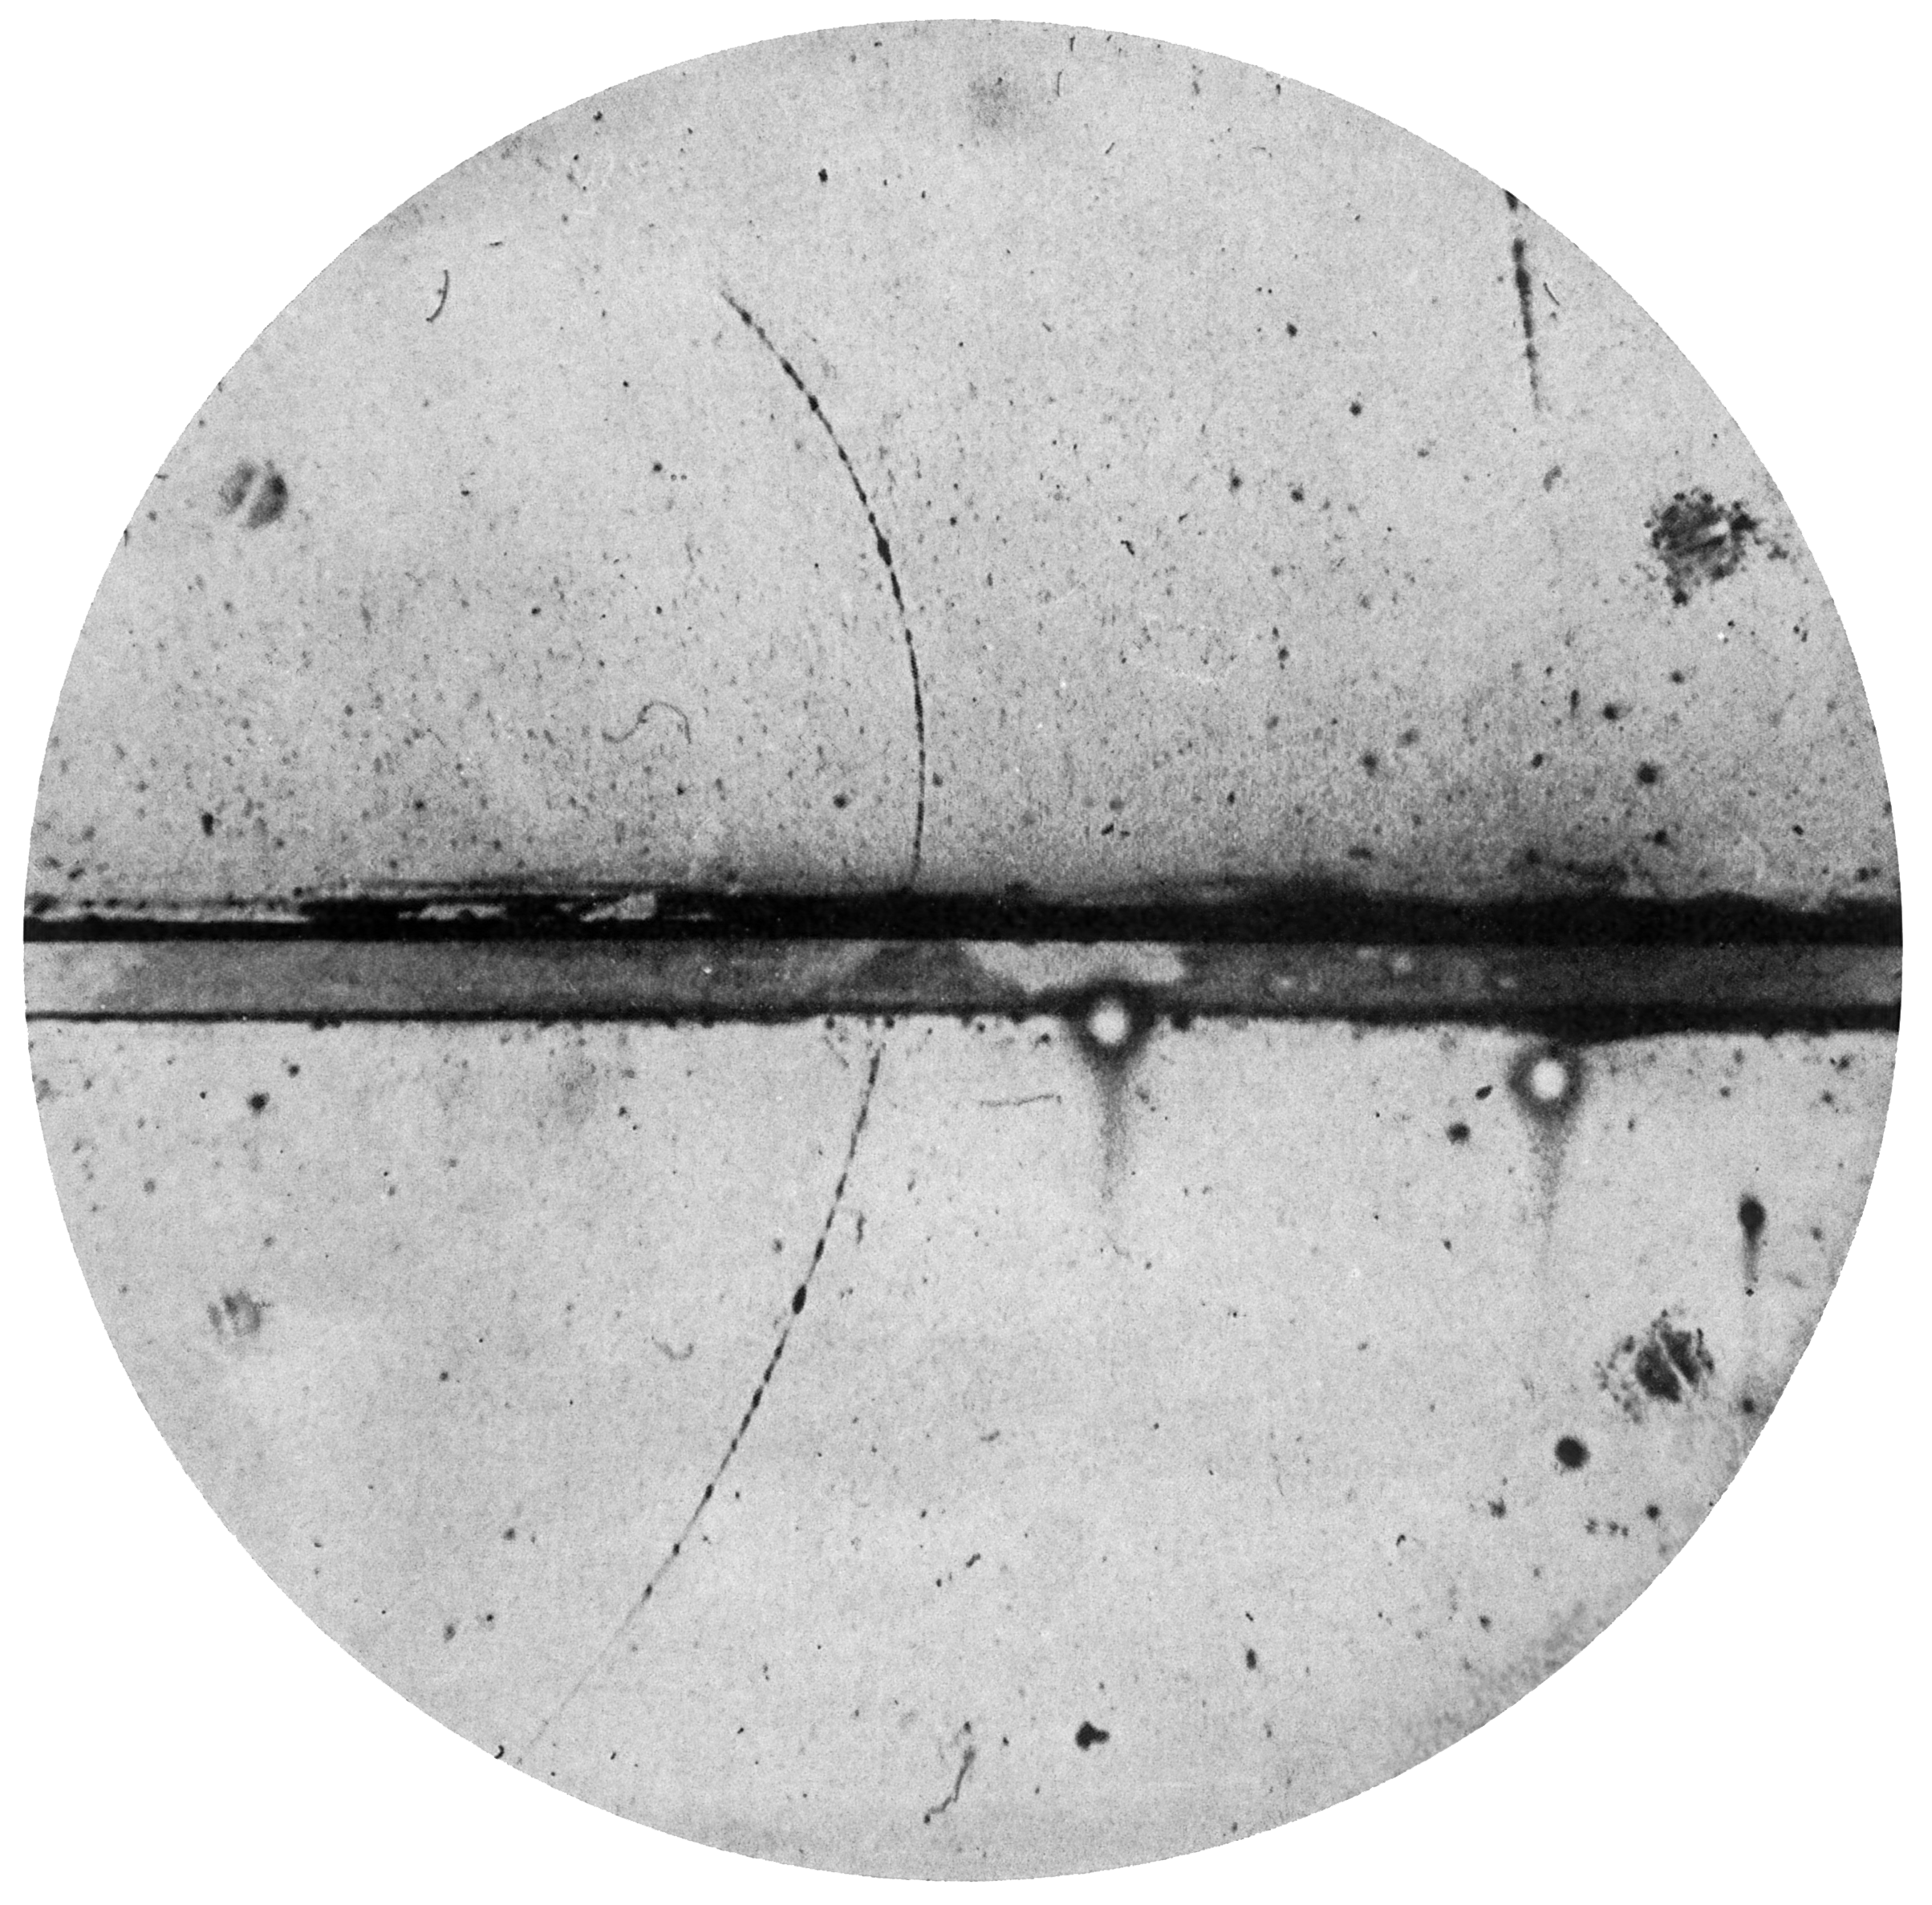
\includegraphics[width=0.55\textwidth]{figures/Part1/Field/Positron}
 \end{tabular}
 \caption{Cloud chamber photograph taken from Anderson's 1932 paper~\cite{PhysRev.43.491}. The upper chamber and the lower chamber are separated by a 6 mm lead plate. The deflection and direction of the particle's ion trail indicate that the particle is a positron.}
 \label{fig:Positron}
 \end{center}
\end{figure}

Quarks participate in all known fundamental interactions and they exist in two different types, up-type and down-type. Up-type and down-type quarks carry $+\frac{2}{3}$ and $-\frac{1}{3}$ electric charges, respectively, in units of the electron charge. For each type of quark, there exist three generations of quarks that are identical copies of each other, except their masses and flavor quantum numbers. For up-type quarks, the three generations are: i) up (u), ii) charm (c), and iii) top (t) quarks. The three generations of up-type quarks are illustrated in the first three columns of the first row in Figure~\ref{fig:Field}. For down-type quarks, the three generations are: i) down (d), ii) strange (s), and iii) bottom (b) quarks. The three generations of down-type quarks are illustrated in the first three columns of the second row in Figure~\ref{fig:Field}. Unlike leptons, which don't interact strongly, quarks carry three types of ``color'' charges: red, green, and blue, which allow them to participate in strong interactions. Strong interactions are discussed in more detail in \autoref{chap:QCD}.

With the exception of top quarks, which decay before forming bound states, quarks are only observed in bound states called ``hadrons'' as stable particles must be color neutral, and carry an integer electric charge. A quark can form two-particle bound states called ``mesons'' with another antiquark with opposite color charges. In addition to two-particle bound states, quarks can also form three- or more-particle bound states. The three-particle bound states, such as a proton (uud), are known as ``baryons''. Bound states with more than three quarks are extremely unstable with a short lifetime, such as the pentaquark recently discovered by the \ac{LHCb} experiment~\cite{LHCb:2015yax}. Because isolated quarks do not exist in nature, their existence must be inferred from the decay products of high-energy collisions. Historically, lighter quarks were observed first as the production of heavier quarks requires higher energy. For example, the existence of charm quarks was confirmed in 1974 at Brookhaven~\cite{E598:1974sol} and SLAC~\cite{SLAC-SP-017:1974ind} (illustrated in Figure~\ref{fig:JPsi}) while top quarks were only observed in 1995 at the Tevatron~\cite{CDF:1995wbb,D0:1995jca}.

\begin{figure}[tbh!]
 \begin{center}
 \begin{tabular}{c}
 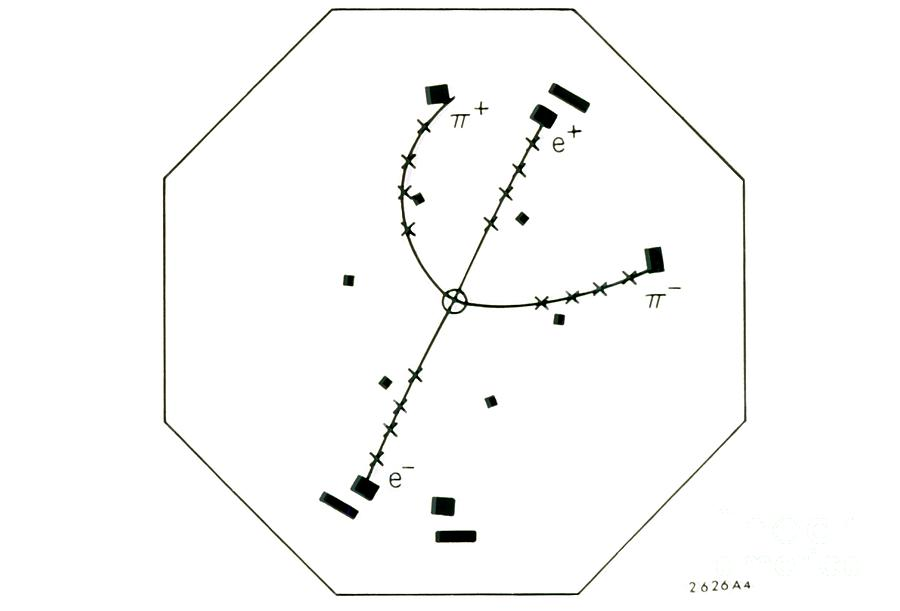
\includegraphics[width=0.7\textwidth]{figures/Part1/Field/J}
 \end{tabular}
 \caption{An example of the $\psi^{\prime}\rightarrow\psi\pi^{+}\pi^{-}$ decay recorded by the Mark I detector in the discovery of $\psi$ particle at SLAC~\cite{SLAC-SP-017:1974ind}. A new resonance around 3.1 GeV was reported by this experiment which was later confirmed to be a two-particle bound state consisting of charm and anticharm quarks.}
 \label{fig:JPsi}
 \end{center}
\end{figure}

Leptons are divided into charged leptons and neutral leptons. Charged leptons carry $-1$ electric charge while neutral leptons, as the name suggests, do not carry any electric charge. Charged leptons participate in electromagnetism and weak interactions while neutral leptons only participate in weak interactions. Similar to quarks, charged- and neutral-leptons exist in three generations, also referred to as ``flavors''. For charged leptons, the three flavors are: i) electron (e), ii) muon ($\upmu$), and iii) tau ($\uptau$). The three flavors of charged leptons are illustrated in the first three columns of the third row in Figure~\ref{fig:Field}. Neutral-leptons are known as ``neutrinos'', which are considered massless in the \ac{SM}. The three flavors of neutrinos are: i) electron neutrino ($\nu_{\textsf{e}}$), ii) muon neutrino ($\nu_{\upmu}$), and iii) tau neutrino ($\nu_{\uptau}$). The three flavors of neutral leptons are illustrated in the first three columns of the fourth row in Figure~\ref{fig:Field}.

Leptons shown in Figure~\ref{fig:Field} have definite masses created by the interaction with Higgs bosons. They are used to describe freely propagating particles of the same mass and quantum numbers, referred to as the ``mass eigenstates''. The three flavors of charged-leptons correspond exactly to their mass eigenstates, which means charged-lepton flavor is conserved in weak interactions. For neutrinos, however, their flavor eigenstates are not identical to their mass eigenstates, which allows neutrinos to oscillate between flavors as they propagate through space. The topic of fermion flavor is discussed further in \autoref{sec:Flavor}. 

The tau lepton is the only lepton that can decay into hadrons (through weak interactions), owing to its higher mass relative to other leptons. The higher mass also means more energy is needed to produce tau leptons. After a decade-long hunt, the tau lepton was eventually detected in 1974 at SLAC~\cite{Perl:1975bf}. Neutrinos only interact weakly, making it virtually impossible to detect them using any general-purpose detectors. It wasn't until the detection of tau neutrinos in 2001 by a dedicated experiment at Fermilab~\cite{DONUT:2000fbd} that all three flavors of neutrinos were experimentally confirmed. 

\section{Bosons}
\label{sec:Boson}

Bosons are named after Indian physicist Satyendra Bose, who along with Einstein, developed the foundations for Bose-Einstein statistics, which states that identical integer spin particles may occupy the same quantum state simultaneously. Elementary bosons in the \ac{SM} consist of spin-1 bosons, which behave like a vector under Lorentz transformation, and scalar bosons with a spin of 0. Vector bosons can be massive or massless and they are mediators of the fundamental forces. For example, photons are quanta of the massless vector boson field that mediates the electromagnetism between charged particles. The particle nature of photons was first demonstrated by American physicist Arthur Compton through the scattering of X-rays in 1923~\cite{PhysRev.21.483}.

The theory that describes the light-matter interaction is known as \ac{QED}, which was first formulated by Dirac in the 1920s. \ac{QED} introduces a photon field by adding two terms to the Dirac Lagrangian,

\begin{equation}
\label{eq:QED}
\mathcal{L}_{QED}=-\frac{1}{4}F_{\mu\nu}F^{\mu\nu}+i\bar{\psi}\gamma^{\mu}\partial_{\mu}\psi-m\bar{\psi}\psi-e\bar{\psi}\gamma^{\mu}A_{\mu}\psi,
\end{equation}

where the first term in Equation~(\ref{eq:QED}) is known as the Electromagnetic tensor, which characterizes the spacetime properties, or more formally the curvature form of the photon field. The last term in Equation~(\ref{eq:QED}) describes the interaction between the fermion fields, mediated by the photon field. 

However, it was soon realized that Dirac's theory was reliable only at a first order of perturbation theory. Attempts to compute high-order processes were often met with \ac{UV} divergence that were nonphysical. This problem remained unsolved for more than 20 years until the Second World War broke out, after which a procedure known as ``renormalization'' was developed independently by Japanese physicist Shinichiro Tomonaga~\cite{Tomonaga:1946zz}, American physicists Julian Schwinger~\cite{Schwinger:1948iu}, and Richard Feynman~\cite{Feynman:1950ir}. Schwinger also provided in his paper a one-loop calculation of the electron anomalous magnetic moment which matched precisely with experiments. British physicist Freeman Dyson also made important contributions by providing mathematical insights into this new technique, most notably demonstrating the equivalence between the seemingly different approaches of Feynman, Schwinger, and Tomonaga~\cite{Dyson:1949bp}. Renormalization was initially designed to systematically remove infinities that appeared in \ac{QED}. It was eventually accepted as a foundational element of quantum field theory as it ensures the validity of physics predictions at different scales. Another key feature of the \ac{QED}, known as gauge invariance, is discussed in \autoref{sec:Gauge}.

Discovered at DESY in 1979~\cite{TASSO:1979zyf}, the gluon is the second elementary boson to be observed experimentally. Like photons, gluons arise from a massless boson field with spin 1. They mediate and participate in the strong interaction as they carry color charge themselves. This property enables the self-interaction of gluons which differentiates itself from the photon. This also means that isolated gluons do not exist in nature as stable particles need to be colorless. The theory of strong interaction is known as \ac{QCD}, which is discussed further in \autoref{chap:QCD}.

Massive vector bosons exist in three types, W$^{+}$, W$^{-}$, and Z bosons. The Z boson has no electric charge while the W$^{+}$ and W$^{-}$ bosons carry the opposite electric charge and are antiparticles of each other. Together, they are also known as weak bosons as they mediate the weak interaction. Weak bosons are among the heaviest fundamental particles in the \ac{SM}, behind only the top quark and the Higgs boson. The heavy mass limits the range of the weak interaction and also raises the threshold energy needed to produce them at high-energy experiments. The existence of these weak bosons was predicted by physicists in the 1960s and was confirmed nearly two decades later by experiments at \ac{CERN} in 1983~\cite{UA1:1983crd,UA2:1983tsx,UA1:1983mne,UA2:1983mlz}. The theory developed by Weinberg that provided a unified description of electromagnetism and weak interaction is discussed further in \autoref{chap:SM}.

The only known elementary boson with spin 0 is the Higgs boson, which was predicted in 1964~\cite{PhysRevLett.13.321,PhysRevLett.13.508,PhysRevLett.13.585} by six physicists including Peter Higgs whose name was given to this massive scalar boson. The Higgs boson is the second heaviest fundamental particle, behind only the top quark. It has no electric charge and its associated Higgs field only interacts with other massive fields with the coupling strength proportional to the particle mass. The Higgs field provides a mechanism to generate mass for other massive fundamental particles, which is discussed further in \autoref{sec:Higgs}. The high mass and lack of quantum charge make Higgs boson extremely difficult to produce. The search for this particle has been one of the longest in history, lasting over 40 years until its eventual observation in 2012 at the \ac{LHC}~\cite{ATLAS:2012yve,CMS:2012qbp}. Evidence for Higgs to two photons presented by the \ac{ATLAS} and \ac{CMS} Collaborations in 2012 is shown in Figure~\ref{fig:Hgg}.

\begin{figure}[tbh!]
 \begin{center}
 \begin{minipage}[b]{0.5\linewidth} 
 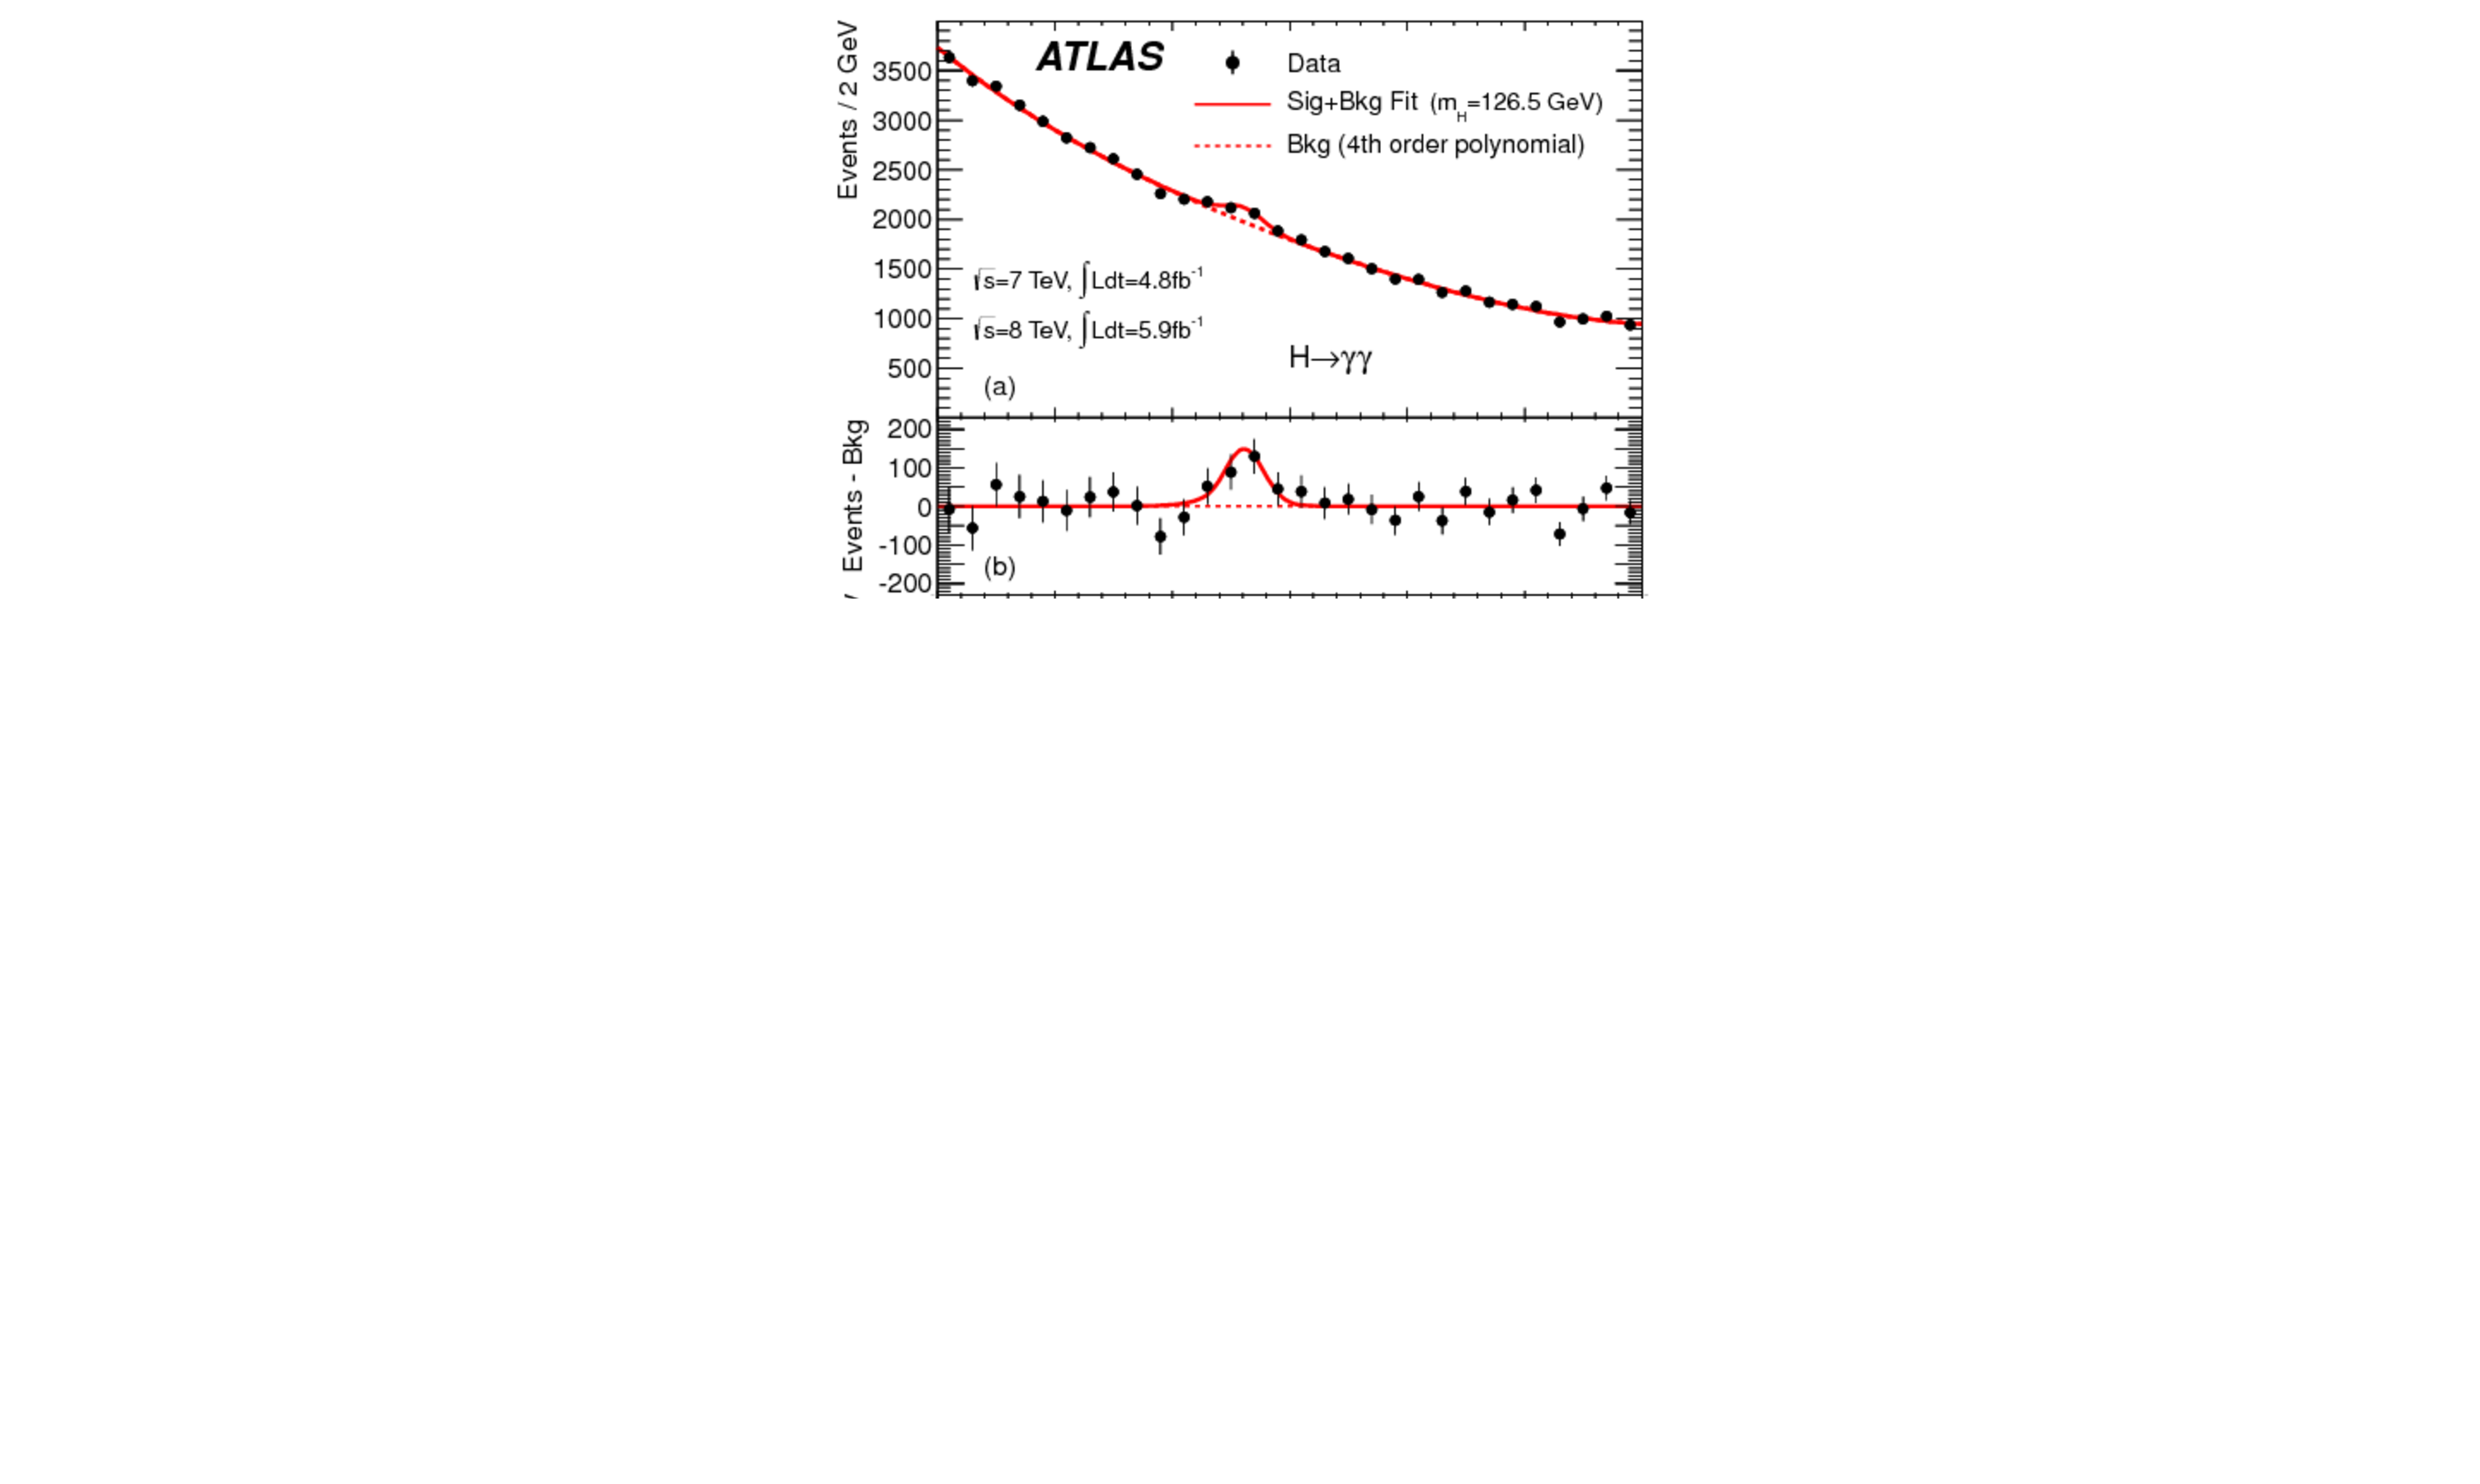
\includegraphics[width=\textwidth]{figures/Part1/Field/ATLAS} 
 \vspace{1em}
 \end{minipage}
 \hfill
 \begin{minipage}[b]{0.45\linewidth} 
 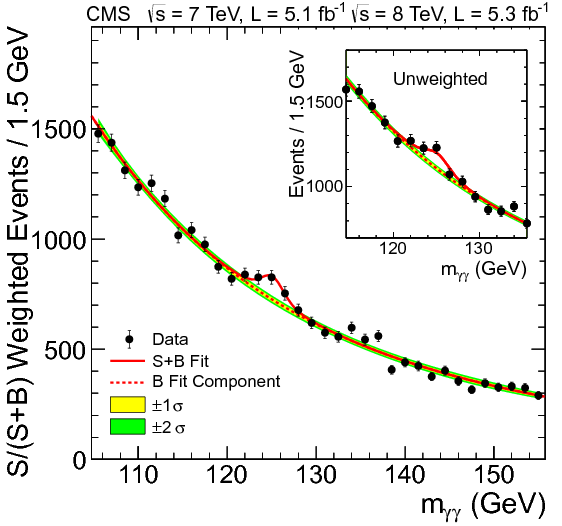
\includegraphics[width=\textwidth]{figures/Part1/Field/CMS}
 \end{minipage}
 \caption{The diphoton invariant mass distributions reported by the \ac{ATLAS}~\cite{ATLAS:2012yve} (left) and \ac{CMS}~\cite{CMS:2012qbp} (right) in their searches for the Higgs boson in 2012. The observed signal around the 125 GeV bump was consistent with the hypothesis of a new massive boson with spin 0, which was later confirmed to be the Higgs boson.}
 \label{fig:Hgg}
 \end{center}
\end{figure}